\chapter{WMAN, The Journey Continues}
\program{WMAN}

\section{Introduction}
\label{ch23-intro}%hyperlabel{ch23-intro}%

At the end of the previous
article I promised that we would continue our look at the standard window definition from
where we left off. In this article that is exactly what we shall be doing as we take a
look into the lists of objects that hang off of our window. I'm referring to the
information sub-{}windows, loose items and applications sub-{}window lists. In addition, we
have also to consider the various objects that are used within these lists.

\section{WMAN Standard Windows Definition -{} Continued}
\label{ch23-std-windef-cntd}%hyperlabel{ch23-std-windef-cntd}%

At the end of the previous article, we had reached the following
definition for our example window:

\begin{lstlisting}[firstnumber=1,caption={WMAN Example Window}]
; Main window definition.
           dc.w  160                ; Default window width
           dc.w  84                 ; Height
           dc.w  146                ; Initial pointer x position 
           dc.w  8                  ; Y position
           dc.b  $00                ; MSbit clear to call CLS
           dc.b  2                  ; Shadow depth 
           dc.w  1                  ; Border width 
           dc.w  0                  ; Border colour (black)
           dc.w  7                  ; Paper colour (white)
           dc.w  0                  ; Use default pointer

; Loose item attributes.
           dc.w  1                  ; Current item border width  
           dc.w  0                  ; Border colour (black)

; Loose item unavailable.
           dc.w  30                 ; Paper - green/white stipple
           dc.w  30                 ; Ink colour 
           dc.w  0                  ; Pointer to blob for pattern
           dc.w  0                  ; Pointer to pattern for blob

; Loose item available.
           dc.w  7                  ; Paper colour (white)
           dc.w  0                  ; Ink colour (black)
           dc.w  0                  ; Pointer to blob for pattern
           dc.w  0                  ; Pointer to pattern for blob

; Loose item selected.
           dc.w  4                  ; Paper colour (green)
           dc.w  0                  ; Ink colour (black)
           dc.w  0                  ; Pointer to blob for pattern
           dc.w  0                  ; Pointer to pattern for blob

; Help window, if used.
           dc.w  0                  ; Pointer to help window

; Repeated part of window definition - from largest to smallest layout.
           dc.w  160                ; Width for this layout
           dc.w  84                 ; Height for this layout

; Pointers to definition lists for this layout.
           dc.w  infoList-*         ; Info sub-windows 
           dc.w  loosList-*         ; Loose items
           dc.w  appList-*          ; App sub-windows

           dc.w  -1                 ; End of layouts
\end{lstlisting}

In this article, we will be concentrating on the final part of the above.

Before we move on, a little light relief. If I replace the pointers to the three
lists in the final part of the layout definition above, with zero -{} to indicate that I have
no loose items, information sub-{}windows or application sub-{}windows -{} and then run the
resulting code, the following screenshot in \figurename~\ref{fig:FirstWindowInAction} shows what I get.

\begin{figure}[h]
\center
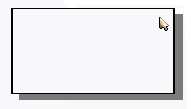
\includegraphics{Content/images/SystemInfo_1.png}
\caption{Basic WMAN Window}
\label{fig:FirstWindowInAction}
\end{figure}

You can see that so far, all we have defined is a small white window, with a shadow
and a black border. The pointer we are using is the default arrow and it is positioned
close to the top at the far right of the window. At least it works!

\begin{note}
You will not be able to assemble the code I have given you so far. There is a
lot more coding to do before you get to that stage. I have a test harness wrapped around
my window definition to make things easier for me to explain as I go along.
\end{note}

\subsection{Information Sub-{}Window List}
\label{ch23-info-windows}%hyperlabel{ch23-info-windows}%

Most PE programs that I have ever seen have a caption bar across the top, possibly
with a few loose items such as sleep (ZZz), Move and so on. The caption bar is usually -{}
but not always -{} green and white stripes with the program name displayed in the middle on
a white background. There are surprisingly, very few programs that do not stick to this
colour scheme, however, the new graphics drivers are changing this and we are starting to
get multi-{}coloured programs with trendy new 3D effects.

That sort of thing can wait until we get to grips with the basics, and so, in the
age old traditions of green and white stripes, we shall continue! In addition, the fancy
effects are only for those of us running SMSQ and so on, they are not available to the
128KB Standard Black Box QL users.

The usual method of getting the green and white caption bar is to define an
information sub-{}window that covers the required length of the window and position it at
the top of the window layout we are defining. The white background for the program name is
simply a second information sub-{}window positioned over the first one. Finally, the title
of the program itself is a text \emph{object} that the second (plain white)
information sub-{}window is linked to. 

To be accurate, the program title is a text string embedded within a text object
linked to the second information sub-{}window. All will become clear below.

The process could almost be likened to the following SuperBasic code.

\begin{lstlisting}[firstnumber=1,language={},caption={Pseudo SuperBasic Equivalent},label={lst:PseudoSuperBasicEquivalent}]
1000 REMark Main Window
1010 OPEN #3,con_
1020 WINDOW #3,160,84,50,32
1030 PAPER #3,7
1040 BORDER #3,1,0
1050 CLS #3
1060 :
1070 REMark Caption Bar background
1080 :
1090 WINDOW #3,98,14,50+30,32+0+1
1100 PAPER #3,85
1110 CLS #3
1120 :
1130 REMark Caption Bar White Bit
1140 :
1150 WINDOW #3,52,10,50+54,32+3+1
1160 PAPER #3,7
1170 INK #3,0
1180 CLS #3
1190 :
1200 REMark Program title
1210 :
1220 PRINT #3,' SysInfo'
1230 :
1240 CLOSE #3
\end{lstlisting}

It isn't quite the same as that, but things should hopefully become clear as we
progress. For now, the definitions of the information sub-{}windows is shown below and
should look strangely familiar.

\begin{lstlisting}[firstnumber=48,caption={WMAN Example Window - Information Window 0}]

; Information sub-window No. 0
infoList dc.w  98                   ; Sub-window width
         dc.w  14                   ; Sub-window height
         dc.w  30                   ; Sub-window x origin
         dc.w  0                    ; Sub-window y origin
         dc.b  $00                  ; MSbit clear to clear window
         dc.b  0                    ; Shadow depth 
         dc.w  0                    ; Border width 
         dc.w  0                    ; Border colour
         dc.w  85                   ; Paper colour (green/white)
         dc.w  0                    ; Pointer to info object list
\end{lstlisting}

Most of the above you have seen before in the fixed part of the main window
definition. As mentioned in the previous article, the shadow depth for sub-{}windows must be
zero. If you are like me, you'll be wondering what happens if you define a shadow on a
sub-{}window. It appears, nothing. I tried putting a shadow of size 1 on an information sub-{}
window and it simply was not drawn. I suspect that internally, WMAN\program{WMAN} is making as many
sanity checks as it can and is probably ignoring the shadow size.

The definition above is equivalent to lines 1070 to 1120 in the SuperBasic code
in Listing~\ref{lst:PseudoSuperBasicEquivalent}. That's an awful lot of typing for a simple result!

Next we need to define the second of our information sub-{}windows, the plain white
one used as a background for the title.

\begin{lstlisting}[firstnumber=last,caption={WMAN Example Window - Information Window 1}]

; Information sub-window No. 1
         dc.w  52                   ; Sub-window width
         dc.w  10                   ; Sub-window height
         dc.w  54                   ; Sub-window x origin
         dc.w  3                    ; Sub-window y origin
         dc.b  $00                  ; MSbit clear to clear window
         dc.b  0                    ; Shadow depth
         dc.w  0                    ; Border width 
         dc.w  0                    ; Border colour
         dc.w  7                    ; Paper colour (white)
         dc.w  infoObjs-*           ; Pointer to info object list

         dc.w  -1                   ; End flag
\end{lstlisting}

As this is our final information sub-window, there is a terminating word of -{}1 at the end of the
definition. The one thing to notice in these definitions is a pointer to a list of
information objects. These are explained next.

Setting the information objects list pointer to zero, in the above, and running the resulting
program gives us the window in \figurename~\ref{fig:FirstWindowInAction2}. You can see both of the information sub-{}windows
now, the green and white stripes is the first and the white one is the second. Next we
shall look at adding an information object to the second one.

\begin{figure}[h]
\center
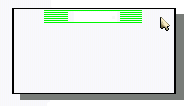
\includegraphics{Content/images/SystemInfo_2.png}
\caption{Basic WMAN Window - With Informations Windows}
\label{fig:FirstWindowInAction2}
\end{figure}


\subsubsection{Information Sub-{}Window Object List}
\label{ch23-info-objects}%hyperlabel{ch23-info-objects}%

There are 4 different types of object that you can place within an information sub-{}
window. These are shown in Table~\ref{tab:InfoSubWindowObjectTypes}.

\begin{table}[htbp]
\centering
\begin{tabular}{l l p{0.7\textwidth}}
\toprule
\textbf{Type} & \textbf{Code} & \textbf{Description} \\
\midrule
Text    &-N & This object is text. Character N will be underlined. \\
Text    & 0 & This object is text. There will be no characters underlined.\\
Sprite  & 2 & This object is a sprite.\\
Blob    & 4 & This object is a blob.\\
Pattern & 8 & This object is a pattern.\\
%
\bottomrule
\end{tabular}
\caption{Information Sub-Window Object Types}
\label{tab:InfoSubWindowObjectTypes}
\end{table}


If the type of the object is negative, then a text object is to be used and the
character in the string corresponding to the negative number `positivised' (I think I just
made up a new word!) will be underlined. We are not using that here, but when we come to
discuss Loose Items, we shall see an example or two.

The following is the definition of our text object for the program title.

\begin{lstlisting}[firstnumber=last,caption={WMAN Example Window - Information Object}]
infoObjs dc.w  42                   ; Object width
         dc.w  10                   ; Object height
         dc.w  6                    ; X origin
         dc.w  0                    ; Y origin
         dc.b  0                    ; Object type (See table)
         dc.b  0                    ; Spare
         dc.w  0                    ; Text ink colour
         dc.b  0                    ; Text character x size
         dc.b  0                    ; Text character y size
         dc.w  prgTitle-*           ; Pointer to object of correct type

         dc.w  -1                   ; end flag
\end{lstlisting}

As we only require one object for our information sub-{}window, there is the usual end
of list indicator word of -{}1 after the definition.

\begin{note}
The information in the following paragraphs has been added by George Gwilt since the original
article was published. These paragraphs correct the original one written by me.\footnote{In \emph{QL Today} Magazine}
\end{note}

If the object is text, the word at offset 10 gives the colour of the ink to be used to display the text. 

If the object is a blob (type 4) the word is used as a word relative pointer to the \emph{pattern} to be used with the blob.

If the object is a pattern (type 6) the word points to the \emph{blob} to be used with the
pattern. 

If the object is a sprite, the word is not used. In all cases the word at offset 14 points to the object itself
whether it is text, sprite, blob or pattern. Thus, for a sprite, its pointer is at offset 14, not 10 as Norman says.


Because this is a text object, we define the ink colour and the character sizes.
However, if the object type is non-{}text ie a blob, pattern or sprite, then the `ink' word
is used as a word sized relative pointer to a pattern or blob or sprite and the character
sizes are ignored. It may be wise to set those to zero just in case.

You will notice that the actual object content is defined elsewhere and one of those
word sized relative pointers (or zero!) is used to tell WMAN\program{WMAN} where the content can be
found.

Because our object is a text object, we simply define a QDSOMSQ format string as
normal and make sure our pointer above actually points to the string. The definition for
our program's title is as follows.

\begin{lstlisting}[firstnumber=last,caption={WMAN Example Window - Information Object Text}]
; Object No. 2       -> TEXT  
prgTitle dc.w  7
         dc.b  'SysInfo'
\end{lstlisting}

Now that we have defined all the required information sub-{}windows and objects that
are required for each, assembling my test program and running it gives the window in \figurename~\ref{fig:FirstWindowInAction3}.

\begin{figure}[h]
\center
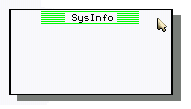
\includegraphics{Content/images/SystemInfo_3.png}
\caption{Basic WMAN Window - With an Information Object}
\label{fig:FirstWindowInAction3}
\end{figure}


Looks much better than the previous plain white version wouldn't you say? You can
see spaces along the caption bar and these will be used -{} very soon -{} for a couple of
loose items. Read on!

\subsection{Loose Item List}
\label{ch23-loose-items}%hyperlabel{ch23-loose-items}%

Loose items are probably the QL's equivalent of Windows Buttons. The following is
the definition of a loose item with a text object displayed upon it.

\begin{lstlisting}[firstnumber=last,caption={WMAN Example Window - Loose Item 0}]
;Loose menu item No. 1
         dc.w  24                   ; Hit area width
         dc.w  11                   ; Height size
         dc.w  132                  ; X origin
         dc.w  2                    ; Y origin
         dc.b  0                    ; Object x justification 
         dc.b  0                    ; Object y justification 
         dc.b  0                    ; Object type
         dc.b  3                    ; Selection keystroke
         dc.w  objESC-*             ; Pointer to object
         dc.w  1                    ; Loose item number
         dc.w  escape-*             ; Pointer to action routine
\end{lstlisting}

You can see a subtle difference between an information sub-{}window and a loose item
definition. Loose items have the properties listed in Table~\ref{tab:LooseItemProperties}.

\begin{table}[htbp]
\centering
\begin{tabular}{p{0.2\textwidth} p{0.7\textwidth}}
\toprule
\textbf{Property} & \textbf{Description} \\
\midrule
%
Hit area width            & The width of the loose item. Includes the border defined above in the fixed definition \\
Hit area height           & The height of the loose item. Includes the border defined above in the fixed definition \\
X origin                  & Where the loose iten will be drawn. Relative to the start of the layout \\
Y origin                  & Where the loose iten will be drawn. Relative to the start of the layout \\
X justification           & How the object will be positioned horozontally within the hit area \\
Y justification           & How the object will be positioned vertically within the hit area \\
Object type               & Same types and rules as for Information sub-window objects above \\
Selection Keystroke       & For a letter, the upper case letter. For an event it is the event number minus 14 \\
Pointer to object         & The usual word sized relative pointer to an object of the correct type. Zero if no text. \\
Loose item number         & The loose item number. You get to choose it. \\
Pointer to action routine & The address of the code to be called when this loose item is HIT or DOne \\
%
\bottomrule
\end{tabular}
\caption{Loose Item Properties}
\label{tab:LooseItemProperties}
\end{table}

As mentioned in Table~\ref{tab:LooseItemProperties}, objects are justified within the loose item hit
area. This is different from the positioning of objects in information sub-{}windows. Table~\ref{tab:LooseItemObjectJustificationRules} shows the justification settings.

\begin{table}[htbp]
\centering
\begin{tabular}{l p{0.7\textwidth}}
\toprule
\textbf{Code} & \textbf{Description} \\
\midrule
%
Positive & The object is left or top justified within the hit area \\
Zero     & The object will be centred within the hit area \\
Negative & The object is right or bottom justified within the hit area \\
%
\bottomrule
\end{tabular}
\caption{Loose Item Object Justification Rules}
\label{tab:LooseItemObjectJustificationRules}
\end{table}

If a key press is required to activate the loose item, it is defined by setting the
code of the capital letter to be used.

\begin{note}
More from George:

First of all, \emph{any} keypress including such things as TAB and the
arrow keys can be used. The selection is not confined to letters and those
keypresses which are defined as `events'. However, lower case letters are not
allowed.
\end{note}

If, on the other hand, some event is to be used to activate the loose item, then the
event number minus 14 is used instead. In our example above, the keystroke is set to 3 for ESC.

If you remember back to Chapter 21 when the event record was described, then you may
get an inkling of what the event number actually is. It is the bit set in the event vector
for the given action. Table~\ref{tab:EventsCodesDescriptions} shows the events and their details.

\begin{table}[htbp]
\centering
\begin{tabular}{l c c p{0.5\textwidth}}
\toprule
\textbf{Event Name} & \textbf{Event Number} & \textbf{Event Code} & \textbf{Description} \\
\midrule
%
DO     & 16 & 2 & ENTER pressed or right mouse button clicked \\
CANCEL & 17 & 3 & ESC pressed \\
HELP   & 18 & 4 & F1 pressed \\
MOVE   & 19 & 5 & CTRL+F4 pressed \\
RESIZE & 20 & 6 & CTRL+F3 pressed \\
SLEEP  & 21 & 7 & CTRL+F1 pressed \\
WAKE   & 22 & 8 & CTRL+F2 pressed \\
%
\bottomrule
\end{tabular}
\caption{Events, Codes and Descriptions}
\label{tab:EventsCodesDescriptions}
\end{table}


\begin{note}
More updates by George.

The official documentation refers to "event number" and "event code". The event number is the number of the bit
set in the event vector which is at position \$14 in the window status area. For the seven events listed by Norman the
corresponding bits to be set are 16 to 22. The event code is the event number less 14. 

If a loose item is to be activated by a keypress producing an event the selection keystroke must be the event
code as Norman says.
\end{note}

The action routine is called when the loose item is HIT or DOne. The parameters
passed to the action routine will be discussed in a later article.

\subsubsection{Loose Item Object List}
\label{ch23-loose-objects}%hyperlabel{ch23-loose-objects}%

Loose item objects are identical to those for information sub-{}windows and so, are
the same to define. The following is an example of the text object required by our example
loose item above.

\begin{lstlisting}[firstnumber=last,caption={WMAN Example Window - Loose Item Object Text}]
; Object No. 4       -> TEXT  
objESC   dc.w  3
         dc.b  'ESC'
\end{lstlisting}

Nothing at all surprising there, it is a text object after all and as such, we
simply define a QDOSMSQ string in the normal manner. Had the object been a blob, pattern
or sprite, we would define one of those in the normal manner. More on those objects later
on in the series.

Now that we have defined all the required loose items and objects that are required
for each, assembling my test program and running it gives the following. I have moved the
pointer from its default position in the screenshot in \figurename~\ref{fig:FirstWindowInAction4} so that you can see the contents of
all the loose items without obstruction.

\begin{figure}[h]
\center
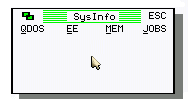
\includegraphics{Content/images/SystemInfo_4.png}
\caption{Basic WMAN Window - With Loose Items}
\label{fig:FirstWindowInAction4}
\end{figure}

All we need now is an application sub-{}window for our code to write to and we are
ready to add actions etc. I shall keep you in suspense until next time.

\section{Coming Up...}
\label{ch23-the-end}%hyperlabel{ch23-the-end}%

In the next chapter we shall continue looking at the remainder of the
standard window definition. It seems like there is quite a lot going on, but it will
hopefully soon be quite easily understood.

We will take a look at adding simple application sub-{}windows and
creating loose item action routines. We might even get a working program to play with, who
knows? See you then.

